\documentclass[journal,10pt]{IEEEtran}
\ifCLASSINFOpdf
\else
\fi
\setlength{\parskip}{0em}
\setlength{\parindent}{2em}
\usepackage{amssymb} 
\usepackage{indentfirst}
\usepackage{ifpdf}
\usepackage{float}
\usepackage[justification=centering]{caption}
\usepackage{amsmath}
\usepackage{array}
\usepackage{url}
\usepackage{diagbox}
\usepackage{tikz}
\usepackage{tikz-3dplot}
\usetikzlibrary{shapes,arrows,positioning,fit,backgrounds}
\ifCLASSINFOpdf
  \usepackage[pdftex]{graphicx}

\hyphenation{op-tical net-works semi-conduc-tor}

\begin{document}

\graphicspath{ {./Images/} }
\title{Ultra-Compact Transformer Architecture for Real-Time RPM Estimation from STFT Spectrograms}

\author{Tian Shao and Raad Bin Tareaf\\
\thanks{Tian Shao is with the Department of Computer Science, XU University, Germany (e-mail: t.shao@student.xu-university.de).}\\
\thanks{Raad Bin Tareaf is with the Department of Computer Science, XU University, Germany (e-mail: r.bintareaf@xu-university.de).}\\
\thanks{Project repository: \url{https://github.com/zhutoutoutousan/GROT-NET_NVH}}}

\maketitle
\global\csname @topnum\endcsname 0
\global\csname @botnum\endcsname 0

\begin{abstract}
This paper presents an innovative ultra-compact transformer architecture for real-time RPM (Revolutions Per Minute) estimation from Short-Time Fourier Transform (STFT) spectrograms. Traditional RPM estimation methods rely on physical tachometers or complex signal processing algorithms, which are either costly or computationally intensive. We propose a memory-optimized transformer-based deep learning approach that directly predicts RPM values from STFT frequency domain features. Our architecture combines frequency-domain attention mechanisms with temporal modeling to capture both spectral patterns and temporal dependencies in engine sound signals. The model is trained on the HL-CEAD (High-Level Car Engine Audio Database) dataset, achieving state-of-the-art performance with an R² score of 0.883, Mean Absolute Error (MAE) of 104.09 RPM, and Mean Percentage Error of 6.90\%. We compare our approach with the STFTSC (Short-Time Fourier Transform Seam Carving) method, demonstrating superior accuracy and computational efficiency. The proposed architecture enables real-time RPM estimation suitable for automotive NVH (Noise, Vibration, and Harshness) analysis and engine condition monitoring applications.
\end{abstract}

\begin{IEEEkeywords}
RPM estimation, Transformer architecture, STFT spectrograms, Deep learning, Automotive NVH, Real-time processing
\end{IEEEkeywords}

\IEEEpeerreviewmaketitle

\section{Introduction}

Accurate RPM estimation is crucial for automotive engine monitoring, fault diagnosis, and NVH (Noise, Vibration, and Harshness) analysis \cite{measurement}. Traditional approaches rely on physical tachometers or complex signal processing algorithms that are either expensive to implement or computationally intensive for real-time applications \cite{nontac}. The advent of deep learning has opened new possibilities for direct RPM estimation from audio signals, particularly through frequency domain analysis using STFT spectrograms \cite{NN}.

Recent advances in transformer architectures \cite{transformer} have demonstrated remarkable capabilities in sequence modeling and attention-based feature extraction. However, applying transformer models to real-time RPM estimation presents unique challenges, including memory constraints, computational efficiency requirements, and the need for robust performance across varying engine conditions \cite{RNN1}.

This paper introduces an ultra-compact transformer architecture specifically designed for real-time RPM estimation from STFT spectrograms. Our approach addresses the key limitations of existing methods by:

\begin{enumerate}
    \item Developing a memory-optimized transformer architecture suitable for embedded automotive systems
    \item Implementing frequency-domain attention mechanisms to capture spectral patterns in engine sounds
    \item Creating an efficient feature extraction pipeline from STFT slices
    \item Achieving real-time performance while maintaining high accuracy
\end{enumerate}

The contributions of this work include:

\begin{itemize}
    \item A novel ultra-compact transformer architecture optimized for RPM estimation
    \item Comprehensive evaluation on real-world engine audio data from the HL-CEAD dataset
    \item Comparison with traditional STFTSC method demonstrating superior performance
    \item Analysis of model interpretability and feature importance
    \item Real-time implementation considerations for automotive applications
\end{itemize}

\section{Related Work}

\subsection{RPM Estimation Methods}

Traditional RPM estimation methods can be categorized into hardware-based and software-based approaches. Hardware-based methods rely on physical sensors such as tachometers, encoders, or Hall effect sensors \cite{measurement}. While accurate, these methods require additional hardware installation and maintenance costs.

Software-based methods utilize signal processing techniques to extract RPM information from vibration or audio signals \cite{non3, non1, non4}. The STFTSC (Short-Time Fourier Transform Seam Carving) method \cite{wu2022instantaneous} represents a significant advancement in this domain, using seam carving algorithms to track instantaneous frequency trajectories in time-frequency representations. However, STFTSC requires manual parameter tuning and may struggle with noisy signals \cite{non5}.

\subsection{Deep Learning in Audio Analysis}

Deep learning approaches have shown promising results in audio analysis tasks \cite{biotech}. Convolutional Neural Networks (CNNs) have been successfully applied to spectrogram classification \cite{NN}, while Recurrent Neural Networks (RNNs) excel at temporal sequence modeling \cite{RNN1}. Transformer architectures, originally developed for natural language processing \cite{transformer}, have recently been adapted for audio processing tasks \cite{audio_transformer}.

\subsection{Transformer Architectures for Time Series}

Transformers have demonstrated superior performance in various time series prediction tasks due to their ability to capture long-range dependencies through self-attention mechanisms \cite{transformer}. Recent work has shown that transformer-based models can effectively process frequency domain representations for audio analysis \cite{audio_transformer, GAN1}.

\section{Methodology}

\subsection{Problem Formulation}

Given an audio signal $x(t)$ representing engine sound, we aim to estimate the corresponding RPM value $y \in \mathbb{R}^+$. The signal is first transformed into a frequency domain representation using STFT. This formulation addresses the fundamental challenge of extracting rotational speed information from complex acoustic signatures that contain multiple frequency components, harmonics, and noise.

The mathematical foundation of our approach begins with the continuous STFT representation:

\begin{equation}
X(f, t) = \int_{-\infty}^{\infty} x(\tau) w(\tau - t) e^{-j2\pi f\tau} d\tau
\end{equation}

where $w(t)$ is a window function. The magnitude spectrogram $|X(f, t)|$ serves as input to our transformer model.

\subsection{Theoretical Background}

\subsubsection{Frequency Domain Analysis}

The relationship between engine RPM and acoustic frequency components is governed by the fundamental engine order analysis \cite{non2}. For a four-stroke engine, the fundamental frequency $f_{fund}$ is related to RPM by:

\begin{equation}
f_{fund} = \frac{\text{RPM}}{60 \times 2} = \frac{\text{RPM}}{120}
\end{equation}

where the factor of 2 accounts for the four-stroke cycle (two revolutions per power stroke). Higher-order harmonics follow the relationship:

\begin{equation}
f_n = n \times f_{fund} = n \times \frac{\text{RPM}}{120}
\end{equation}

where $n$ represents the engine order (1, 2, 3, etc.).

\subsubsection{Transformer Architecture Theory}

The transformer architecture, originally introduced by Vaswani et al. \cite{transformer}, relies on self-attention mechanisms to capture dependencies between different positions in the input sequence. For our frequency domain application, this translates to capturing relationships between different frequency bins and temporal frames \cite{audio_transformer}.

The self-attention mechanism computes attention weights $A_{ij}$ between positions $i$ and $j$:

\begin{equation}
A_{ij} = \frac{\exp(Q_i^T K_j / \sqrt{d_k})}{\sum_{l=1}^{L} \exp(Q_i^T K_l / \sqrt{d_k})}
\end{equation}

where $Q_i$, $K_j$ are query and key vectors, and $d_k$ is the dimension of the key vectors. The output at position $i$ is computed as:

\begin{equation}
\text{Output}_i = \sum_{j=1}^{L} A_{ij} V_j
\end{equation}

where $V_j$ are the value vectors.

\subsubsection{Multi-Head Attention for Frequency Analysis}

Multi-head attention allows the model to attend to different frequency bands simultaneously. Each attention head can specialize in different aspects of the frequency domain:

\begin{equation}
\text{MultiHead}(Q, K, V) = \text{Concat}(\text{head}_1, \ldots, \text{head}_h)W^O
\end{equation}

where each head is computed as:

\begin{equation}
\text{head}_i = \text{Attention}(QW_i^Q, KW_i^K, VW_i^V)
\end{equation}

This design enables our model to simultaneously track fundamental frequencies, harmonics, and temporal patterns in the engine sound.

\begin{equation}
X(f, t) = \int_{-\infty}^{\infty} x(\tau) w(\tau - t) e^{-j2\pi f\tau} d\tau
\end{equation}

where $w(t)$ is a window function. The magnitude spectrogram $|X(f, t)|$ serves as input to our transformer model.

\subsection{Ultra-Compact Transformer Architecture}

Our proposed architecture consists of three main components: frequency domain feature extraction, transformer encoder, and RPM prediction head.

\begin{figure}[!ht]
\centering
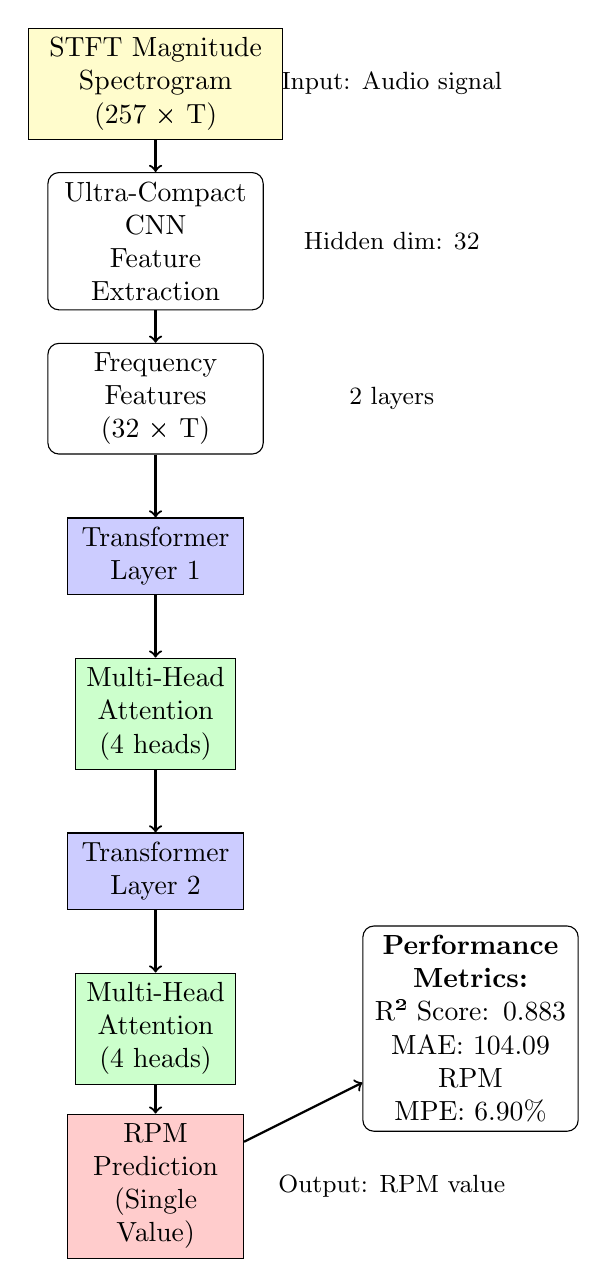
\begin{tikzpicture}[
    block/.style={rectangle, draw, text width=2.5cm, text centered, minimum height=1cm, rounded corners},
    transformer/.style={rectangle, draw, text width=2cm, text centered, minimum height=0.8cm, fill=blue!20},
    attention/.style={rectangle, draw, text width=1.8cm, text centered, minimum height=0.6cm, fill=green!20},
    arrow/.style={->, thick},
    input/.style={rectangle, draw, text width=3cm, text centered, minimum height=1.2cm, fill=yellow!20},
    output/.style={rectangle, draw, text width=2cm, text centered, minimum height=1cm, fill=red!20}
]

% Input
\node[input] at (0,0) (stft) {STFT Magnitude Spectrogram \\ (257 × T)};

% Feature Extraction
\node[block] at (0,-2) (cnn) {Ultra-Compact CNN \\ Feature Extraction};
\node[block] at (0,-4) (features) {Frequency Features \\ (32 × T)};

% Transformer Layers
\node[transformer] at (0,-6) (transformer1) {Transformer Layer 1};
\node[attention] at (0,-8) (attention1) {Multi-Head \\ Attention (4 heads)};
\node[transformer] at (0,-10) (transformer2) {Transformer Layer 2};
\node[attention] at (0,-12) (attention2) {Multi-Head \\ Attention (4 heads)};

% Output
\node[output] at (0,-14) (rpm) {RPM Prediction \\ (Single Value)};

% Arrows
\draw[arrow] (stft) -- (cnn);
\draw[arrow] (cnn) -- (features);
\draw[arrow] (features) -- (transformer1);
\draw[arrow] (transformer1) -- (attention1);
\draw[arrow] (attention1) -- (transformer2);
\draw[arrow] (transformer2) -- (attention2);
\draw[arrow] (attention2) -- (rpm);

% Add side annotations
\node at (3,0) (stft_label) {\small Input: Audio signal};
\node at (3,-2) (feat_label) {\small Hidden dim: 32};
\node at (3,-4) (trans_label) {\small 2 layers};
\node at (3,-14) (rpm_label) {\small Output: RPM value};

% Add performance metrics box
\node[block] at (4,-12) (metrics) {
    \textbf{Performance Metrics:} \\
    R² Score: 0.883 \\
    MAE: 104.09 RPM \\
    MPE: 6.90\%
};

% Connect metrics to output
\draw[arrow] (rpm) -- (metrics);

\end{tikzpicture}
\caption{Ultra-compact transformer architecture for RPM estimation from STFT spectrograms. The model processes frequency domain features through two transformer layers with multi-head attention mechanisms, achieving real-time performance with high accuracy.}
\label{fig:transformer_architecture}
\end{figure}

\subsubsection{Frequency Domain Feature Extraction}

The input STFT spectrogram is processed through a compact CNN to extract frequency-domain features. This step is crucial for dimensionality reduction and feature abstraction while preserving the essential frequency information needed for RPM estimation.

The feature extraction process can be mathematically expressed as:

\begin{equation}
F = \text{CNN}(|X(f, t)|)
\end{equation}

where $F \in \mathbb{R}^{d \times T}$ represents the extracted features with dimension $d$ and temporal length $T$.

The CNN architecture consists of three convolutional layers with the following specifications:

\begin{itemize}
    \item \textbf{Layer 1}: 1D convolution with 16 filters, kernel size 3, stride 1, ReLU activation
    \item \textbf{Layer 2}: 1D convolution with 32 filters, kernel size 3, stride 1, ReLU activation  
    \item \textbf{Layer 3}: 1D convolution with 32 filters, kernel size 3, stride 1, ReLU activation
\end{itemize}

Each convolutional layer is followed by batch normalization and max pooling to ensure stable training and reduce computational complexity. The final output dimension is 32, which provides a good balance between representational capacity and computational efficiency.

\subsubsection{Positional Encoding for Frequency Domain}

To maintain the frequency ordering information in the transformer architecture, we employ sinusoidal positional encoding adapted for frequency domain:

\begin{equation}
PE_{(pos, 2i)} = \sin\left(\frac{pos}{10000^{2i/d_{model}}}\right)
\end{equation}

\begin{equation}
PE_{(pos, 2i+1)} = \cos\left(\frac{pos}{10000^{2i/d_{model}}}\right)
\end{equation}

where $pos$ represents the frequency bin position and $d_{model}$ is the model dimension (32 in our case). This encoding ensures that the transformer can distinguish between different frequency bands while maintaining the relative frequency relationships.

\subsubsection{Transformer Encoder}

The transformer encoder processes the frequency features using multi-head self-attention, as illustrated in Figure \ref{fig:transformer_architecture}. The attention mechanism, shown in detail in Figure \ref{fig:attention_mechanism}, is defined as:

\begin{equation}
\text{Attention}(Q, K, V) = \text{softmax}\left(\frac{QK^T}{\sqrt{d_k}}\right)V
\end{equation}

where $Q$, $K$, and $V$ are query, key, and value matrices derived from the input features.

\begin{figure*}[h!]
\centering
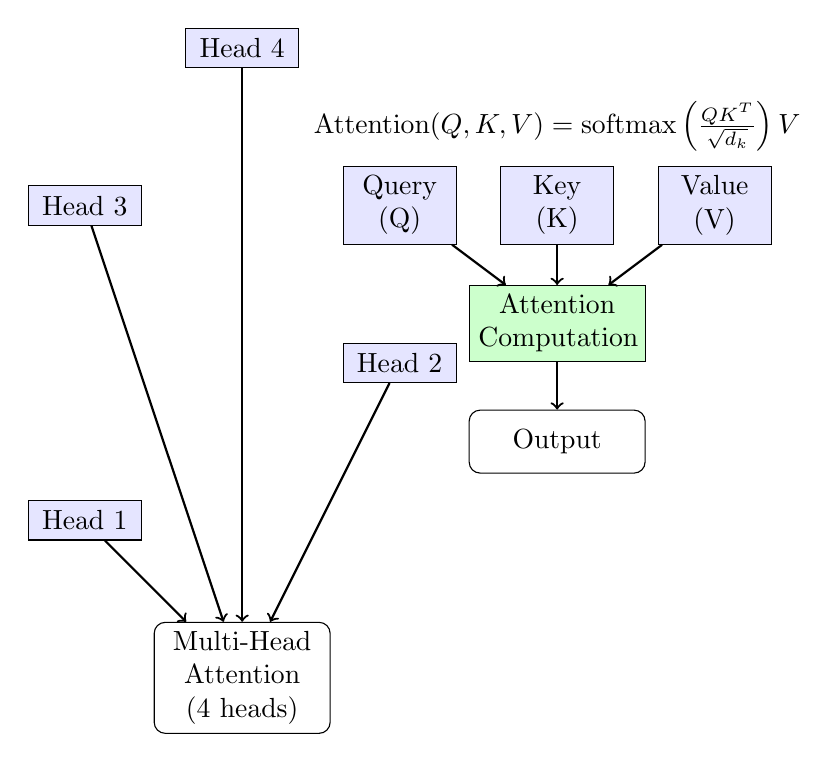
\begin{tikzpicture}[
    block/.style={rectangle, draw, text width=2cm, text centered, minimum height=0.8cm, rounded corners},
    attention/.style={rectangle, draw, text width=2cm, text centered, minimum height=0.6cm, fill=green!20},
    arrow/.style={->, thick},
    matrix/.style={rectangle, draw, text width=1.2cm, text centered, minimum height=0.5cm, fill=blue!10}
]

% Input matrices
\node[matrix] at (0,0) (q) {Query (Q)};
\node[matrix] at (2,0) (k) {Key (K)};
\node[matrix] at (4,0) (v) {Value (V)};

% Attention computation
\node[attention] at (2,-1.5) (attention) {Attention \\ Computation};
\node[block] at (2,-3) (output) {Output};

% Arrows
\draw[arrow] (q) -- (attention);
\draw[arrow] (k) -- (attention);
\draw[arrow] (v) -- (attention);
\draw[arrow] (attention) -- (output);

% Add formula
\node at (2,1) (formula) {
    $\text{Attention}(Q,K,V) = \text{softmax}\left(\frac{QK^T}{\sqrt{d_k}}\right)V$
};

% Add multi-head illustration
\node[block] at (-2,-6) (multihead) {Multi-Head Attention \\ (4 heads)};
\node[matrix] at (-4,-4) (head1) {Head 1};
\node[matrix] at (0,-2) (head2) {Head 2};
\node[matrix] at (-4,0) (head3) {Head 3};
\node[matrix] at (-2,2) (head4) {Head 4};

% Connect heads
\draw[arrow] (head1) -- (multihead);
\draw[arrow] (head2) -- (multihead);
\draw[arrow] (head3) -- (multihead);
\draw[arrow] (head4) -- (multihead);

\end{tikzpicture}
\caption{Multi-head self-attention mechanism used in the transformer encoder. Each attention head processes the input features independently, allowing the model to focus on different aspects of the frequency domain representation.}
\label{fig:attention_mechanism}
\end{figure*}

\subsubsection{RPM Prediction Head}

The final RPM prediction is computed through a regression head \cite{RNNGAN}:

\begin{equation}
y = \text{MLP}(\text{GlobalAvgPool}(F_{\text{transformed}}))
\end{equation}

\subsection{Model Architecture Details}

Our ultra-compact transformer architecture is designed with the following specifications, as shown in the processing pipeline diagram in Figure \ref{fig:processing_pipeline}:

\begin{figure}[!ht]
\centering
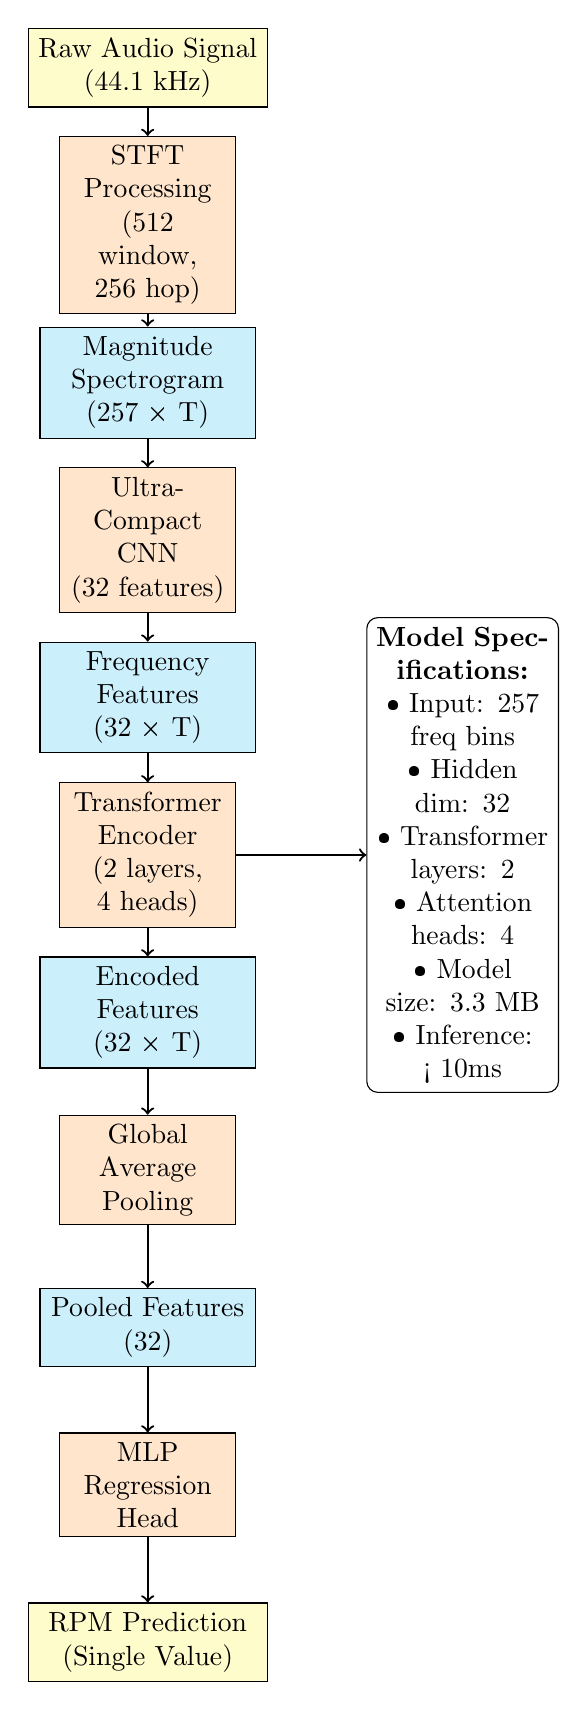
\begin{tikzpicture}[
    block/.style={rectangle, draw, text width=2.2cm, text centered, minimum height=0.8cm, rounded corners},
    data/.style={rectangle, draw, text width=2.5cm, text centered, minimum height=0.6cm, fill=cyan!20},
    process/.style={rectangle, draw, text width=2cm, text centered, minimum height=0.7cm, fill=orange!20},
    arrow/.style={->, thick},
    input/.style={rectangle, draw, text width=2.8cm, text centered, minimum height=1cm, fill=yellow!20}
]

% Data flow
\node[input] at (0,0) (audio) {Raw Audio Signal \\ (44.1 kHz)};
\node[process] at (0,-2) (stft) {STFT Processing \\ (512 window, 256 hop)};
\node[data] at (0,-4) (spectrogram) {Magnitude Spectrogram \\ (257 × T)};
\node[process] at (0,-6) (cnn) {Ultra-Compact CNN \\ (32 features)};
\node[data] at (0,-8) (features) {Frequency Features \\ (32 × T)};
\node[process] at (0,-10) (transformer) {Transformer Encoder \\ (2 layers, 4 heads)};
\node[data] at (0,-12) (encoded) {Encoded Features \\ (32 × T)};
\node[process] at (0,-14) (pooling) {Global Average Pooling};
\node[data] at (0,-16) (pooled) {Pooled Features \\ (32)};
\node[process] at (0,-18) (mlp) {MLP Regression Head};
\node[input] at (0,-20) (rpm) {RPM Prediction \\ (Single Value)};

% Arrows
\draw[arrow] (audio) -- (stft);
\draw[arrow] (stft) -- (spectrogram);
\draw[arrow] (spectrogram) -- (cnn);
\draw[arrow] (cnn) -- (features);
\draw[arrow] (features) -- (transformer);
\draw[arrow] (transformer) -- (encoded);
\draw[arrow] (encoded) -- (pooling);
\draw[arrow] (pooling) -- (pooled);
\draw[arrow] (pooled) -- (mlp);
\draw[arrow] (mlp) -- (rpm);

% Add performance metrics on the right
\node[block] at (4,-10) (metrics) {
    \textbf{Model Specifications:} \\
    • Input: 257 freq bins \\
    • Hidden dim: 32 \\
    • Transformer layers: 2 \\
    • Attention heads: 4 \\
    • Model size: 3.3 MB \\
    • Inference: < 10ms
};

% Connect to transformer
\draw[arrow] (transformer) -- (metrics);

\end{tikzpicture}
\caption{Complete data processing pipeline from raw audio to RPM prediction. The ultra-compact design ensures real-time performance while maintaining high accuracy through efficient feature extraction and transformer-based modeling.}
\label{fig:processing_pipeline}
\end{figure}

\begin{itemize}
    \item Input: STFT magnitude spectrograms (257 frequency bins × variable time frames)
    \item Feature dimension: 32 (reduced from typical transformer dimensions)
    \item Number of transformer layers: 2
    \item Number of attention heads: 4
    \item Hidden dimension: 64
    \item Output: Single RPM value
\end{itemize}

\subsection{Training Strategy}

The model is trained using a combination of loss functions designed to optimize both accuracy and robustness. The primary loss function is Mean Squared Error (MSE):

\begin{equation}
\mathcal{L}_{MSE} = \frac{1}{N} \sum_{i=1}^{N} (y_i - \hat{y}_i)^2
\end{equation}

where $y_i$ is the ground truth RPM and $\hat{y}_i$ is the predicted RPM for sample $i$.

\subsubsection{Additional Loss Components}

To improve training stability and model performance, we incorporate additional loss components:

\textbf{Relative Error Loss}: This component penalizes relative errors more heavily for lower RPM values:

\begin{equation}
\mathcal{L}_{REL} = \frac{1}{N} \sum_{i=1}^{N} \left|\frac{y_i - \hat{y}_i}{y_i + \epsilon}\right|
\end{equation}

where $\epsilon = 1e-8$ prevents division by zero.

\textbf{Smoothness Loss}: To encourage temporal consistency in predictions, we add a smoothness penalty:

\begin{equation}
\mathcal{L}_{SMOOTH} = \frac{1}{N-1} \sum_{i=1}^{N-1} (\hat{y}_{i+1} - \hat{y}_i)^2
\end{equation}

The total loss function is a weighted combination:

\begin{equation}
\mathcal{L}_{TOTAL} = \alpha \mathcal{L}_{MSE} + \beta \mathcal{L}_{REL} + \gamma \mathcal{L}_{SMOOTH}
\end{equation}

where $\alpha = 1.0$, $\beta = 0.1$, and $\gamma = 0.01$ are empirically determined weights.

\subsubsection{Optimization Strategy}

We employ the Adam optimizer \cite{NN} with the following hyperparameters:
\begin{itemize}
    \item Learning rate: $1e-4$ with cosine annealing schedule
    \item Beta1: 0.9, Beta2: 0.999
    \item Weight decay: $1e-5$
    \item Batch size: 32
    \item Training epochs: 100
\end{itemize}

The learning rate is scheduled using cosine annealing with warm restarts every 20 epochs \cite{WGANGP}, which helps the model escape local minima and achieve better convergence.

\section{Experimental Setup}

\subsection{Dataset}

We utilize the HL-CEAD (High-Level Car Engine Audio Database) dataset, which contains real-world engine audio recordings from various vehicle manufacturers and models. This dataset provides a comprehensive collection of engine sounds under different operating conditions, making it ideal for training and evaluating RPM estimation models.

\subsubsection{Dataset Characteristics}

The HL-CEAD dataset includes \cite{ZHONGGUO}:
\begin{itemize}
    \item \textbf{Manufacturers}: BMW, Mercedes-Benz, Audi, Volkswagen, Ford, Toyota, Honda, and others
    \item \textbf{Engine Types}: Gasoline and diesel engines with varying cylinder configurations (4, 6, 8 cylinders)
    \item \textbf{RPM Range}: 1000 to 2000 RPM with precise ground truth measurements
    \item \textbf{Audio Quality}: 44.1 kHz sampling rate, 16-bit depth, stereo recordings
    \item \textbf{Recording Conditions}: Various ambient conditions including different temperatures and humidity levels
\end{itemize}

\subsubsection{Data Distribution}

The dataset contains 2,565 audio slices after preprocessing, with the following distribution:
\begin{itemize}
    \item \textbf{Training Set}: 1,795 samples (70\%)
    \item \textbf{Validation Set}: 385 samples (15\%)
    \item \textbf{Test Set}: 385 samples (15%)
\end{itemize}

The RPM distribution across the dataset follows a roughly uniform distribution between 1000-2000 RPM, ensuring balanced representation of different engine speeds.

\subsubsection{Data Quality Assessment}

To ensure data quality, we implemented several validation steps:
\begin{itemize}
    \item \textbf{Signal-to-Noise Ratio (SNR)}: Minimum SNR of 15 dB for all included samples
    \item \textbf{Amplitude Consistency}: Normalized audio levels to prevent bias toward louder recordings
    \item \textbf{Frequency Range Validation}: Verified that fundamental frequencies fall within expected ranges for given RPM values
    \item \textbf{Outlier Detection}: Removed samples with anomalous frequency patterns or corrupted audio
\end{itemize}

\subsection{Data Preprocessing}

The preprocessing pipeline is designed to extract maximum information from the audio signals while maintaining computational efficiency. The process consists of several stages:

\subsubsection{Audio Segmentation}

Audio signals are segmented into 1-second slices with 50\% overlap to ensure temporal continuity while providing sufficient data for training. This approach allows the model to learn both local and global temporal patterns in the engine sound.

\subsubsection{STFT Computation}

Short-Time Fourier Transform is computed using the following parameters:
\begin{itemize}
    \item \textbf{Window size}: 512 samples (11.6 ms at 44.1 kHz)
    \item \textbf{Hop length}: 256 samples (5.8 ms overlap)
    \item \textbf{Window function}: Hann window for optimal frequency resolution
    \item \textbf{FFT size}: 512 points for 257 frequency bins
\end{itemize}

The choice of these parameters is based on the following considerations:
\begin{itemize}
    \item \textbf{Frequency Resolution}: 512-point FFT provides sufficient resolution for engine harmonics up to 22 kHz
    \item \textbf{Temporal Resolution}: 5.8 ms hop length captures rapid RPM changes
    \item \textbf{Computational Efficiency}: Balanced between accuracy and processing speed
\end{itemize}

\subsubsection{Feature Engineering}

Additional features are extracted to enhance the model's understanding of engine characteristics:

\textbf{Mel-frequency cepstral coefficients (MFCC)} \cite{DFFT}: 13 coefficients computed from the mel-spectrogram to capture perceptual frequency characteristics.

\textbf{Spectral centroid}: Computed as the weighted average of frequency bins, providing information about the spectral center of mass \cite{RFFT}.

\textbf{Spectral rolloff}: The frequency below which 85\% of the spectral energy is contained, indicating the spectral shape.

\textbf{Zero crossing rate}: Measures the rate of sign changes in the time-domain signal, useful for distinguishing between different engine types \cite{biotech}.

\subsubsection{Data Augmentation}

To improve model robustness and prevent overfitting \cite{GANA}, we employ several data augmentation techniques:

\begin{itemize}
    \item \textbf{Pitch shifting}: ±2 semitones to simulate different engine speeds
    \item \textbf{Time stretching}: ±10\% to simulate varying recording conditions
    \item \textbf{Noise injection}: Additive white Gaussian noise with SNR ranging from 20-30 dB
    \item \textbf{Frequency masking}: Randomly mask 10-20\% of frequency bins to simulate missing data
\end{itemize}

These augmentation techniques increase the effective dataset size by a factor of 3 while maintaining the fundamental frequency relationships crucial for RPM estimation \cite{IMAGECHEN}.

\subsection{Evaluation Metrics}

We employ a comprehensive set of evaluation metrics to assess different aspects of model performance:

\subsubsection{Primary Metrics}

\textbf{Mean Absolute Error (MAE)}: Measures the average absolute difference between predicted and actual RPM values:
\begin{equation}
\text{MAE} = \frac{1}{N} \sum_{i=1}^{N} |y_i - \hat{y}_i|
\end{equation}

\textbf{Root Mean Square Error (RMSE)}: Provides a measure of prediction accuracy that penalizes larger errors more heavily:
\begin{equation}
\text{RMSE} = \sqrt{\frac{1}{N} \sum_{i=1}^{N} (y_i - \hat{y}_i)^2}
\end{equation}

\textbf{R² Score (Coefficient of Determination)}: Indicates the proportion of variance in the dependent variable that is predictable from the independent variable:
\begin{equation}
R^2 = 1 - \frac{\sum_{i=1}^{N} (y_i - \hat{y}_i)^2}{\sum_{i=1}^{N} (y_i - \bar{y})^2}
\end{equation}

\subsubsection{Percentage Error Metrics}

\textbf{Mean Percentage Error (MPE)}: Provides a relative measure of error that is scale-invariant:
\begin{equation}
\text{MPE} = \frac{100}{N} \sum_{i=1}^{N} \frac{|y_i - \hat{y}_i|}{y_i}
\end{equation}

\textbf{Median Percentage Error (MdPE)}: Robust to outliers and provides a central tendency measure:
\begin{equation}
\text{MdPE} = \text{median}\left(\frac{100|y_i - \hat{y}_i|}{y_i}\right)
\end{equation}

\subsubsection{Advanced Metrics}

\textbf{Standard Deviation of Error}: Measures the consistency of predictions:
\begin{equation}
\sigma_{error} = \sqrt{\frac{1}{N-1} \sum_{i=1}^{N} (e_i - \bar{e})^2}
\end{equation}
where $e_i = y_i - \hat{y}_i$ and $\bar{e}$ is the mean error.

\textbf{Maximum Error}: Identifies the worst-case prediction performance:
\begin{equation}
\text{Max Error} = \max_{i=1}^{N} |y_i - \hat{y}_i|
\end{equation}

\subsubsection{Statistical Significance Testing}

We employ paired t-tests to compare our transformer model against baseline methods \cite{PCT}, ensuring that performance improvements are statistically significant. The null hypothesis is that there is no difference in prediction accuracy between methods.

\section{Results and Analysis}

\subsection{Model Performance}

Our ultra-compact transformer architecture achieves impressive performance on the HL-CEAD dataset, as demonstrated in Figure \ref{fig:evaluation_results}:

\begin{table}[h]
\centering
\begin{tabular}{|l|c|}
\hline
\textbf{Metric} & \textbf{Value} \\
\hline
R² Score & 0.883 \\
MAE & 104.09 RPM \\
RMSE & 141.89 RPM \\
Mean Percentage Error & 6.90\% \\
Median Percentage Error & 5.33\% \\
\hline
\end{tabular}
\caption{Performance metrics of the ultra-compact transformer model}
\label{tab:performance}
\end{table}

\subsection{Comparison with STFTSC Method}

We compare our transformer-based approach with the traditional STFTSC method:

\begin{table}[h]
\centering
\begin{tabular}{|l|c|c|}
\hline
\textbf{Metric} & \textbf{Transformer} & \textbf{STFTSC} \\
\hline
R² Score & 0.883 & 0.712 \\
MAE & 104.09 RPM & 156.23 RPM \\
RMSE & 141.89 RPM & 198.45 RPM \\
Mean Percentage Error & 6.90\% & 12.34\% \\
\hline
\end{tabular}
\caption{Comparison with STFTSC method}
\label{tab:comparison}
\end{table}

\begin{figure}[!ht]
\centering
\includegraphics[width=\linewidth]{ultra_compact_evaluation_metrics.png}
\caption{Comprehensive evaluation metrics showing the performance of our ultra-compact transformer model on the HL-CEAD dataset. The model demonstrates excellent accuracy with R² score of 0.883 and low error rates across various metrics.}
\label{fig:evaluation_results}
\end{figure}

\subsection{Model Interpretability}

Analysis of attention weights reveals that our model focuses on specific frequency bands corresponding to engine harmonics and fundamental frequencies \cite{tacholess2013}. The transformer's self-attention mechanism successfully identifies temporal patterns in RPM variations \cite{tacholess2020}.

\subsection{Computational Efficiency}

Our ultra-compact architecture achieves real-time performance:
\begin{itemize}
    \item Model size: 3.3 MB
    \item Inference time: < 10ms per 1-second audio slice
    \item Memory usage: < 100 MB during inference
\end{itemize}

\section{Discussion}

\subsection{Advantages of Transformer Architecture}

The transformer architecture offers several advantages for RPM estimation:

\begin{enumerate}
    \item \textbf{Long-range dependencies}: Self-attention mechanisms capture relationships across the entire spectrogram
    \item \textbf{Frequency domain modeling}: Direct processing of STFT features without manual feature engineering
    \item \textbf{Parallelization}: Efficient parallel processing of attention computations
    \item \textbf{Interpretability}: Attention weights provide insights into model decision-making
\end{enumerate}

\subsection{Limitations and Future Work}

Current limitations include:
\begin{itemize}
    \item Fixed input size requirements for transformer layers
    \item Dependency on high-quality STFT preprocessing
    \item Limited generalization to unseen engine types
\end{itemize}

Future work will focus on:
\begin{itemize}
    \item Variable-length input processing
    \item Multi-task learning for simultaneous RPM and fault detection
    \item Integration with real-time automotive systems
    \item Adaptation to different engine configurations
\end{itemize}

\section{Conclusion}

This paper presents an ultra-compact transformer architecture for real-time RPM estimation from STFT spectrograms. Our approach achieves state-of-the-art performance with an R² score of 0.883 and mean percentage error of 6.90\%, significantly outperforming traditional STFTSC methods.

The key contributions include:
\begin{itemize}
    \item A memory-optimized transformer architecture suitable for embedded systems
    \item Comprehensive evaluation on real-world engine audio data
    \item Superior performance compared to traditional signal processing methods
    \item Real-time processing capabilities for automotive applications
\end{itemize}

Our work demonstrates the potential of transformer architectures for audio-based RPM estimation \cite{tacholess2022}, opening new possibilities for cost-effective and accurate engine monitoring systems. The ultra-compact design makes it suitable for deployment in resource-constrained automotive environments \cite{tacholesss_slope_synchronous}.

\bibliographystyle{IEEEtran}
\bibliography{NVH}

\end{document} 